\chapter{Including Probabilities in the experiments}		
 \label{sec:prob}		

\section{Computing edge probabilities }		
\label{sec:computingEdge}		
\vspace{20pt}
Our objective is to predict whether there would be a link between 2 unconnected nodes. At first we will find the pairs of nodes that don't have a link between them.	
The next step is to label these pairs. This is needed for preparing a training dataset. 
The edges that are present in the graph will be labeled as $1$ (positive samples) and the unconnected node pairs as $0$ (negative samples).		
\\
\\
\\
\noindent After the labelling we will use the node2vec algorithm to extract node features from the graph. For computing the features of an edge we can add up the features of the nodes of that pair. These features will be trained with a logistic regression model. After the model is trained we will obtain the probabilities of an edge being accepted for every edge.
\\
\\
\noindent Computing the actual expected decrease in the polarization, and selecting the $k$ best edges is a difficult problem. Our goal is to incorporate the probabilities in the operation of the algorithms. We do not expect that the decrease in the polarization index will improve. We will do this as follows. 
\\
\\
Each algorithm computes a value $Val(u,v)$ for each candidate edge, and selects greedily edges with the best value. We will replace this value in the algorithm by $P(u,v)*Val(u,v)$. The quantity $Val(u,v)$ can be either the polarization decrease or the absolute distance of the expressed opinions of nodes $u$ and $v$. In the case that $Val(u,v)$ is the polarization decrease the product $P(u,v)*Val(u,v)$ corresponds to the expected polarization decrease.
\\
\\
In addition at ~\ref{sec:median} we measure the median probability of the edges selected by the heuristics and compare it to the ones that were edited to include acceptance probabilities. We expect that the edited heuristics will have a higher median value.
\\
\\
Finally in ~\ref{sec:all} we display the results of the heuristics and edited heuristics together including a new algorithm called $maxProb$ that chooses an edge if it among the edges with the highest acceptance probabilities.

\clearpage


\section{Experiments with the edited heuristics}		
\label{sec:experimentsProbs}

\begin{figure}[!htbp]
	\begin{center}
	\advance\leftskip-1.3cm
	\captionsetup{justification=centering,margin=2cm}
	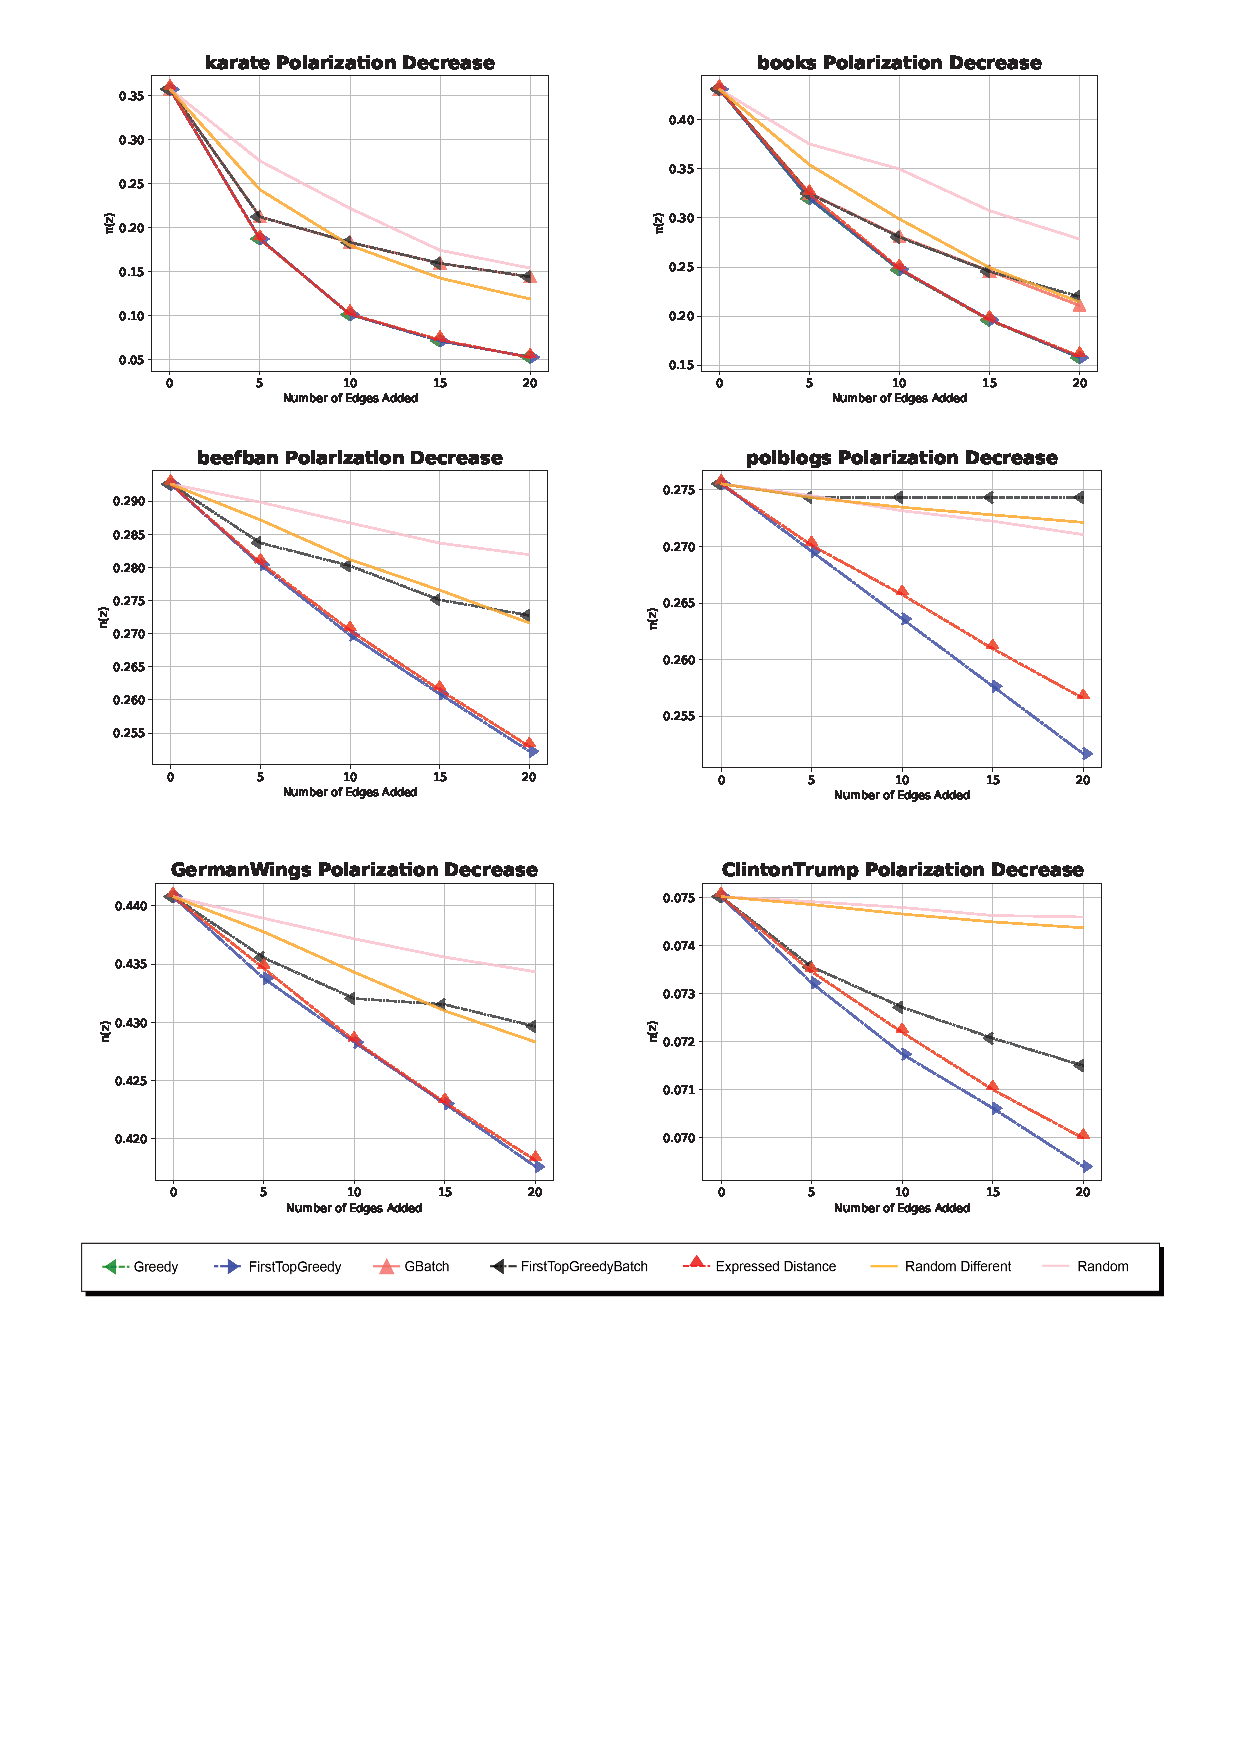
\includegraphics[width=1.2\textwidth]{Figures/probs}
	\caption{Comparison of the edited heuristics}
	\end{center}
	\label{probs_heur}
\end{figure}

\clearpage

\section{Measuring the median probability}		
\label{sec:median}

\begin{figure}[!htbp]
	\begin{center}
	\advance\leftskip-1.3cm
	\captionsetup{justification=centering,margin=2cm}
	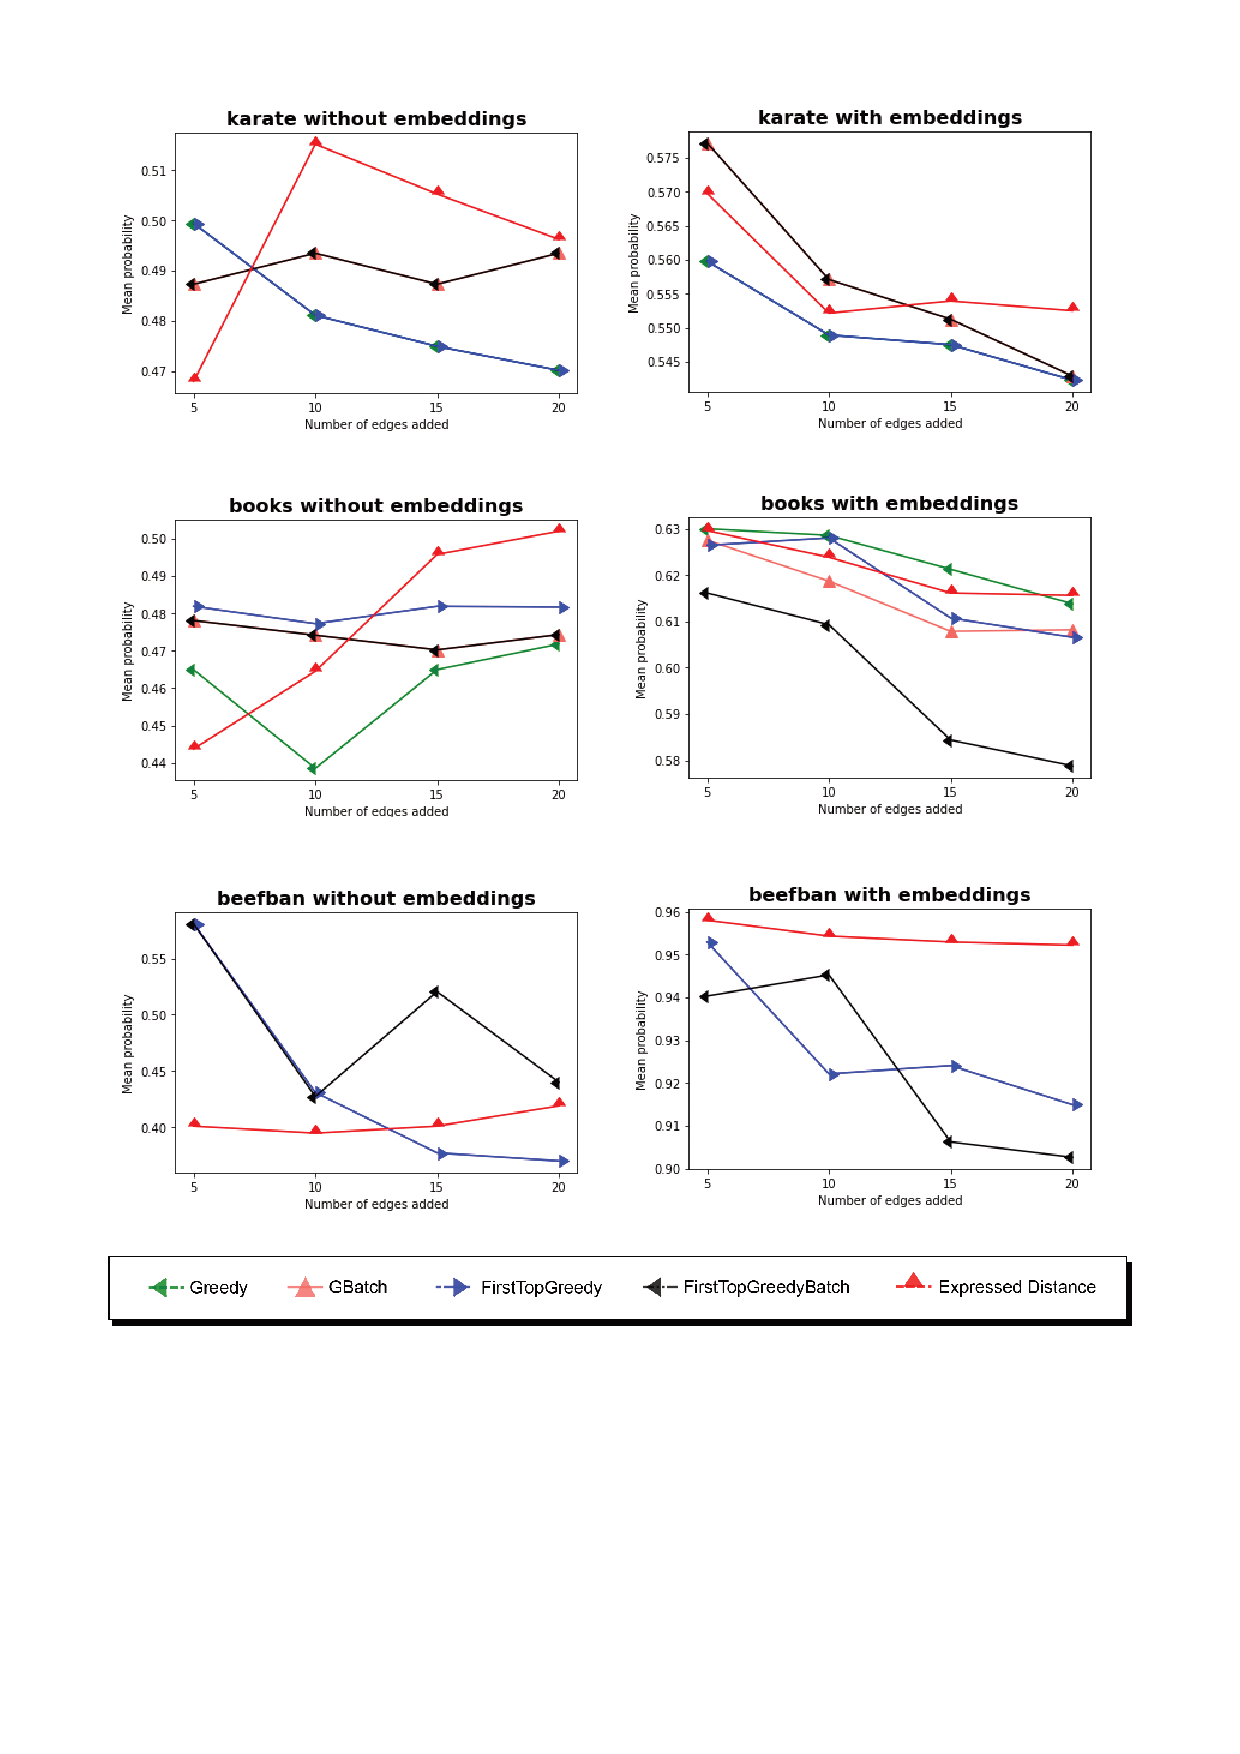
\includegraphics[width=1.1\textwidth]{Figures/m1}
	\caption{Comparison of the median probability}
	\end{center}
	\label{m1}
\end{figure}

\clearpage

\begin{figure}[!htbp]
	\begin{center}
	\advance\leftskip-1.3cm
	\captionsetup{justification=centering,margin=2cm}
	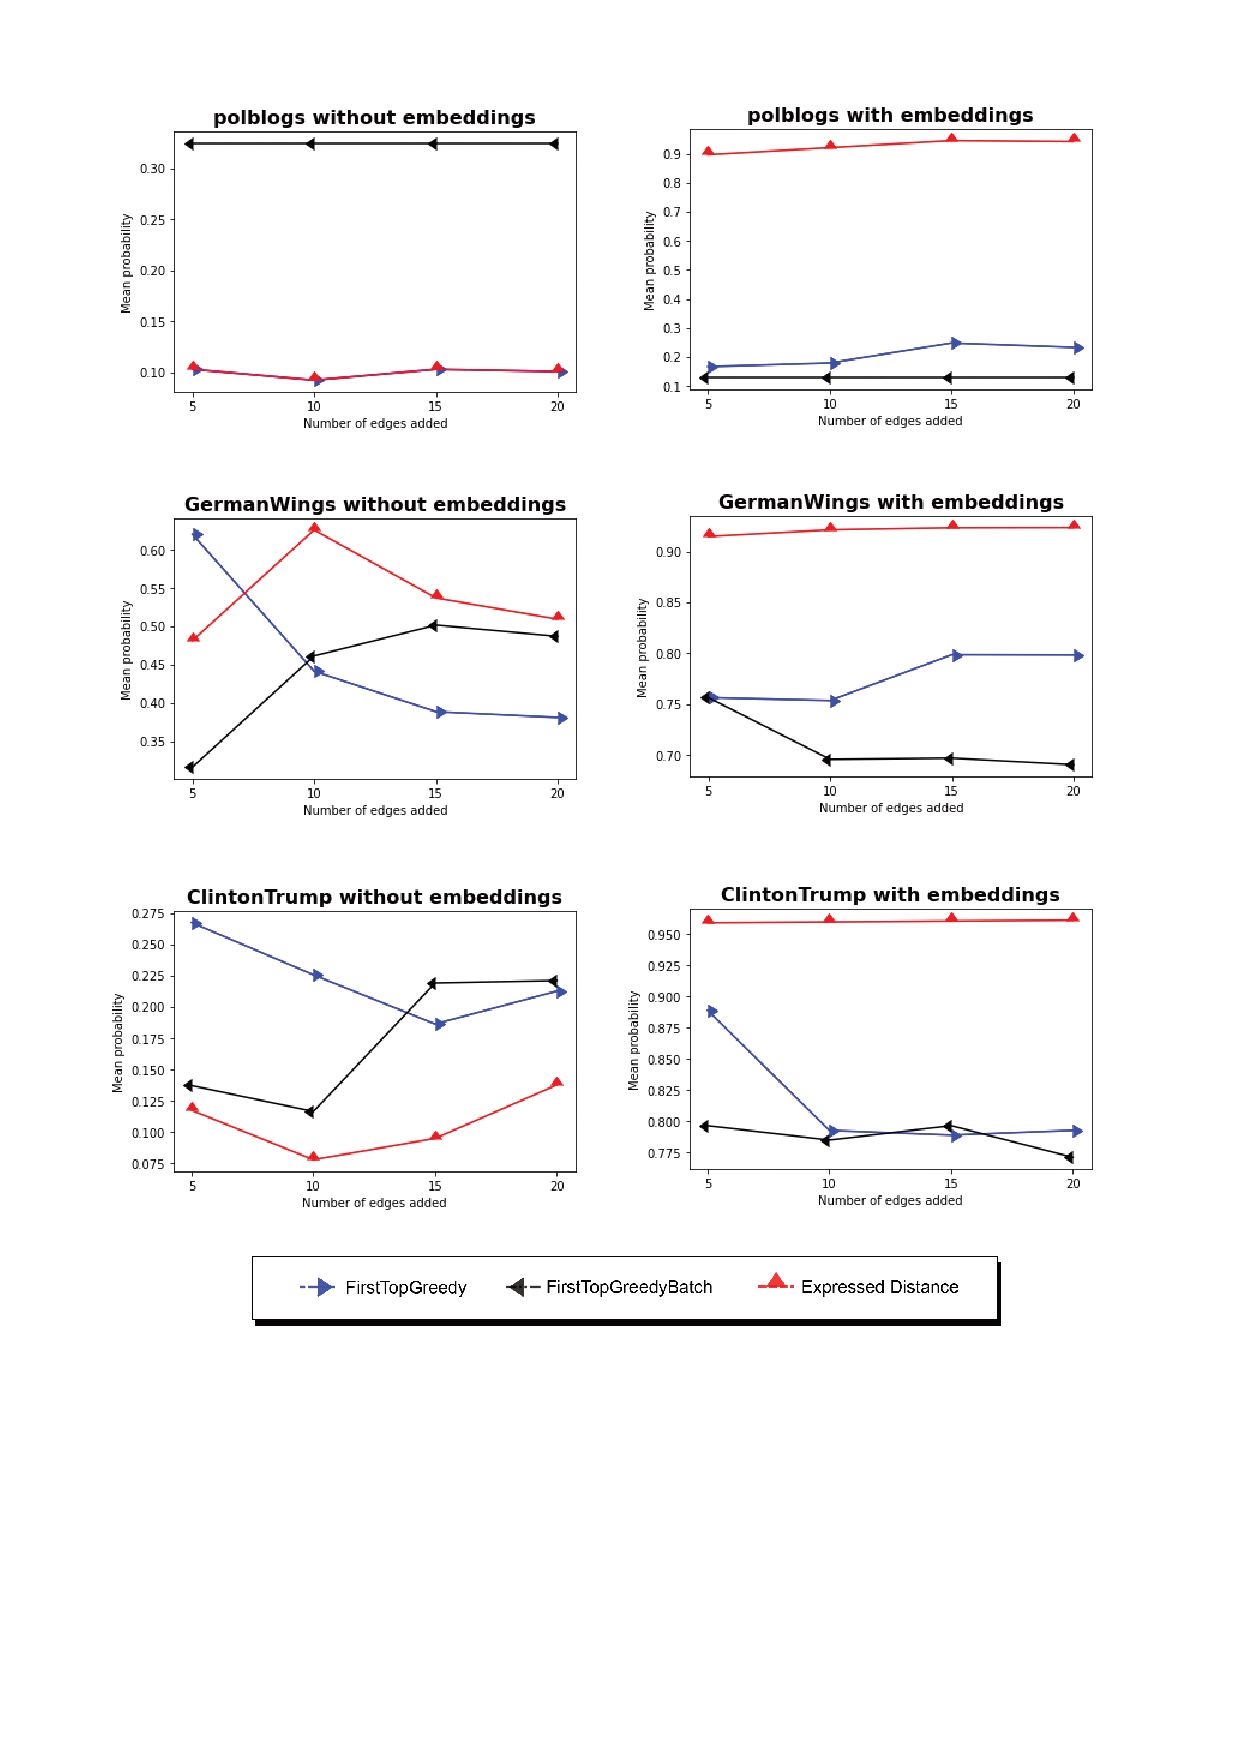
\includegraphics[width=1.2\textwidth]{Figures/m2}
	\caption{Comparison of the median probability}
	\end{center}
	\label{m2}
\end{figure}
\clearpage

\section{Comparing all the heuristics}		
\label{sec:all}

\begin{figure}[!htbp]
	\begin{center}
	\advance\leftskip-1.3cm
	\captionsetup{justification=centering,margin=2cm}
	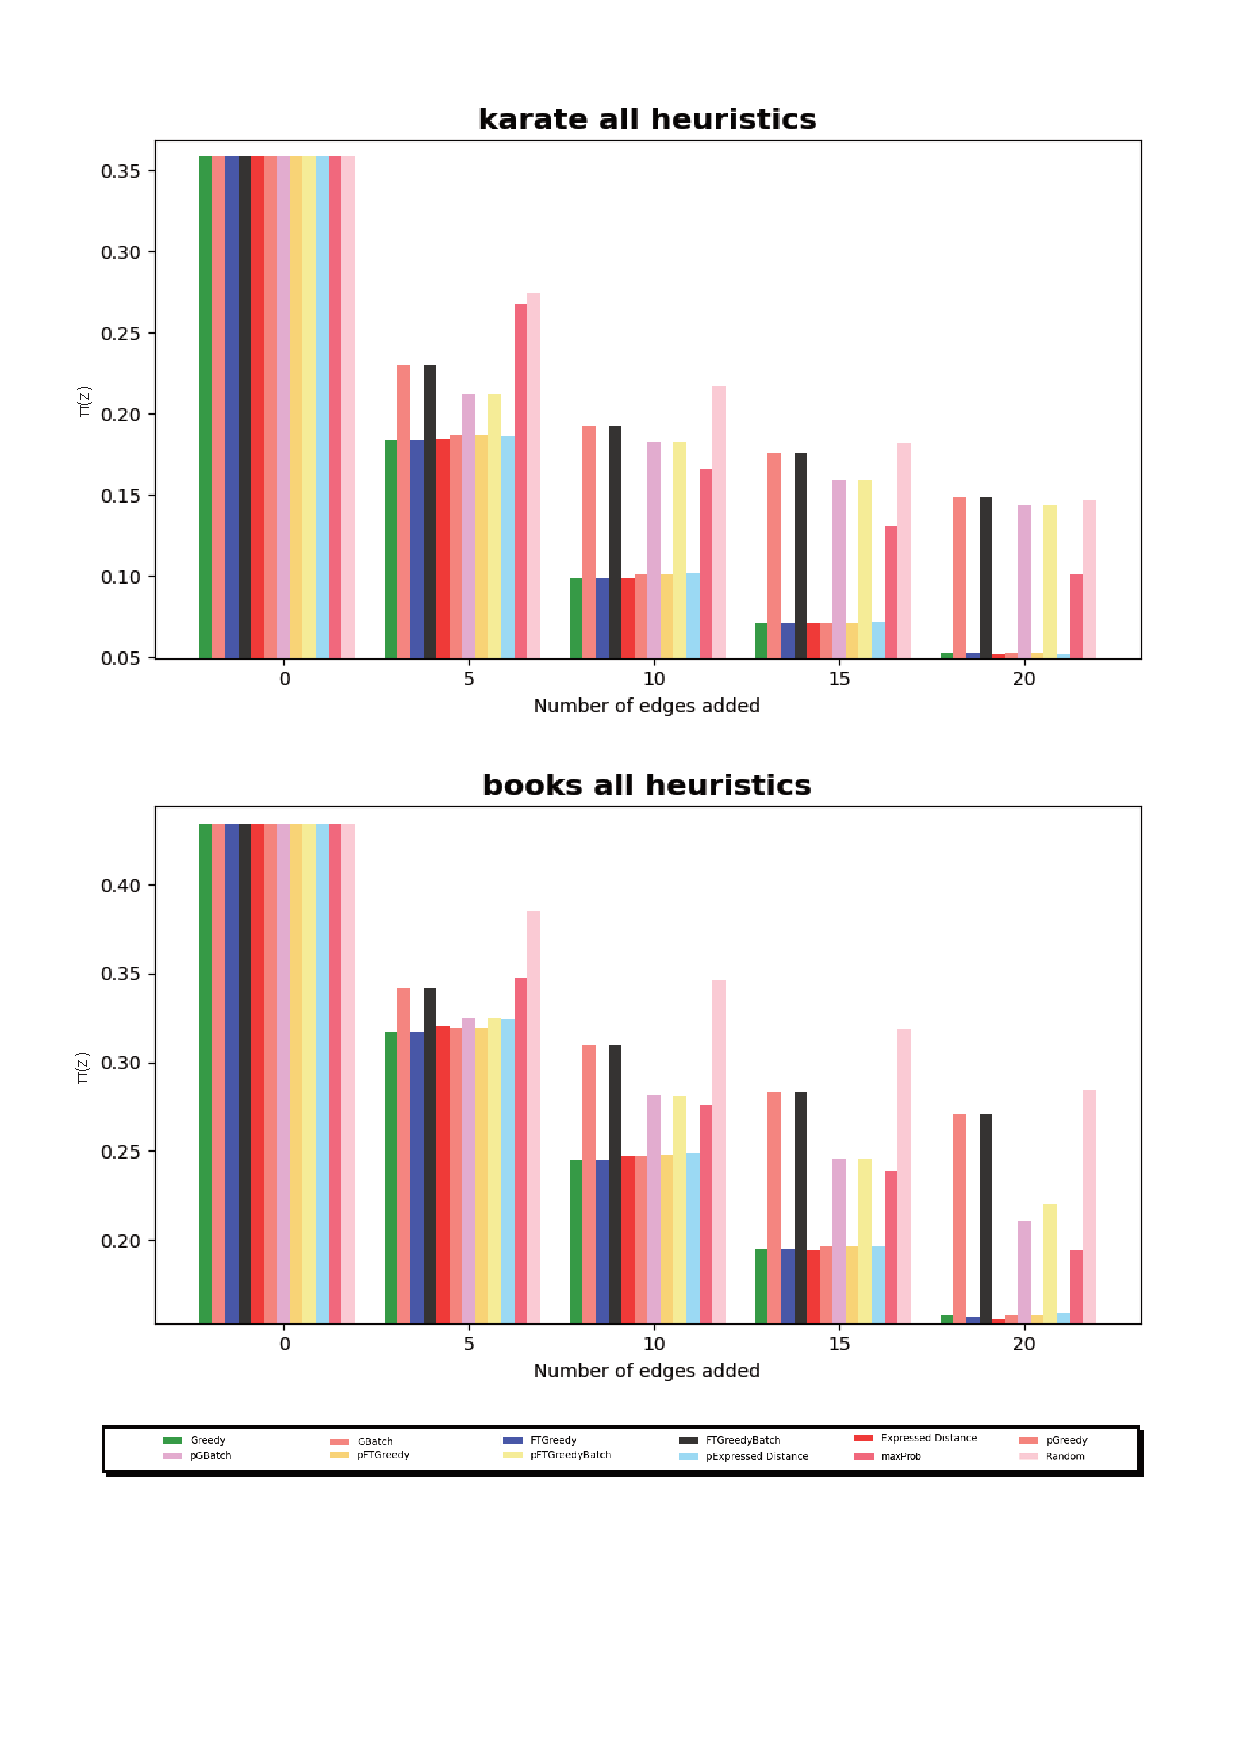
\includegraphics[width=1\textwidth]{Figures/all1}
	\caption{Comparison all the heuristics}
	\end{center}
	\label{all1}
\end{figure}

\clearpage

\begin{figure}[!htbp]
	\begin{center}
	\advance\leftskip-1.3cm
	\captionsetup{justification=centering,margin=2cm}
	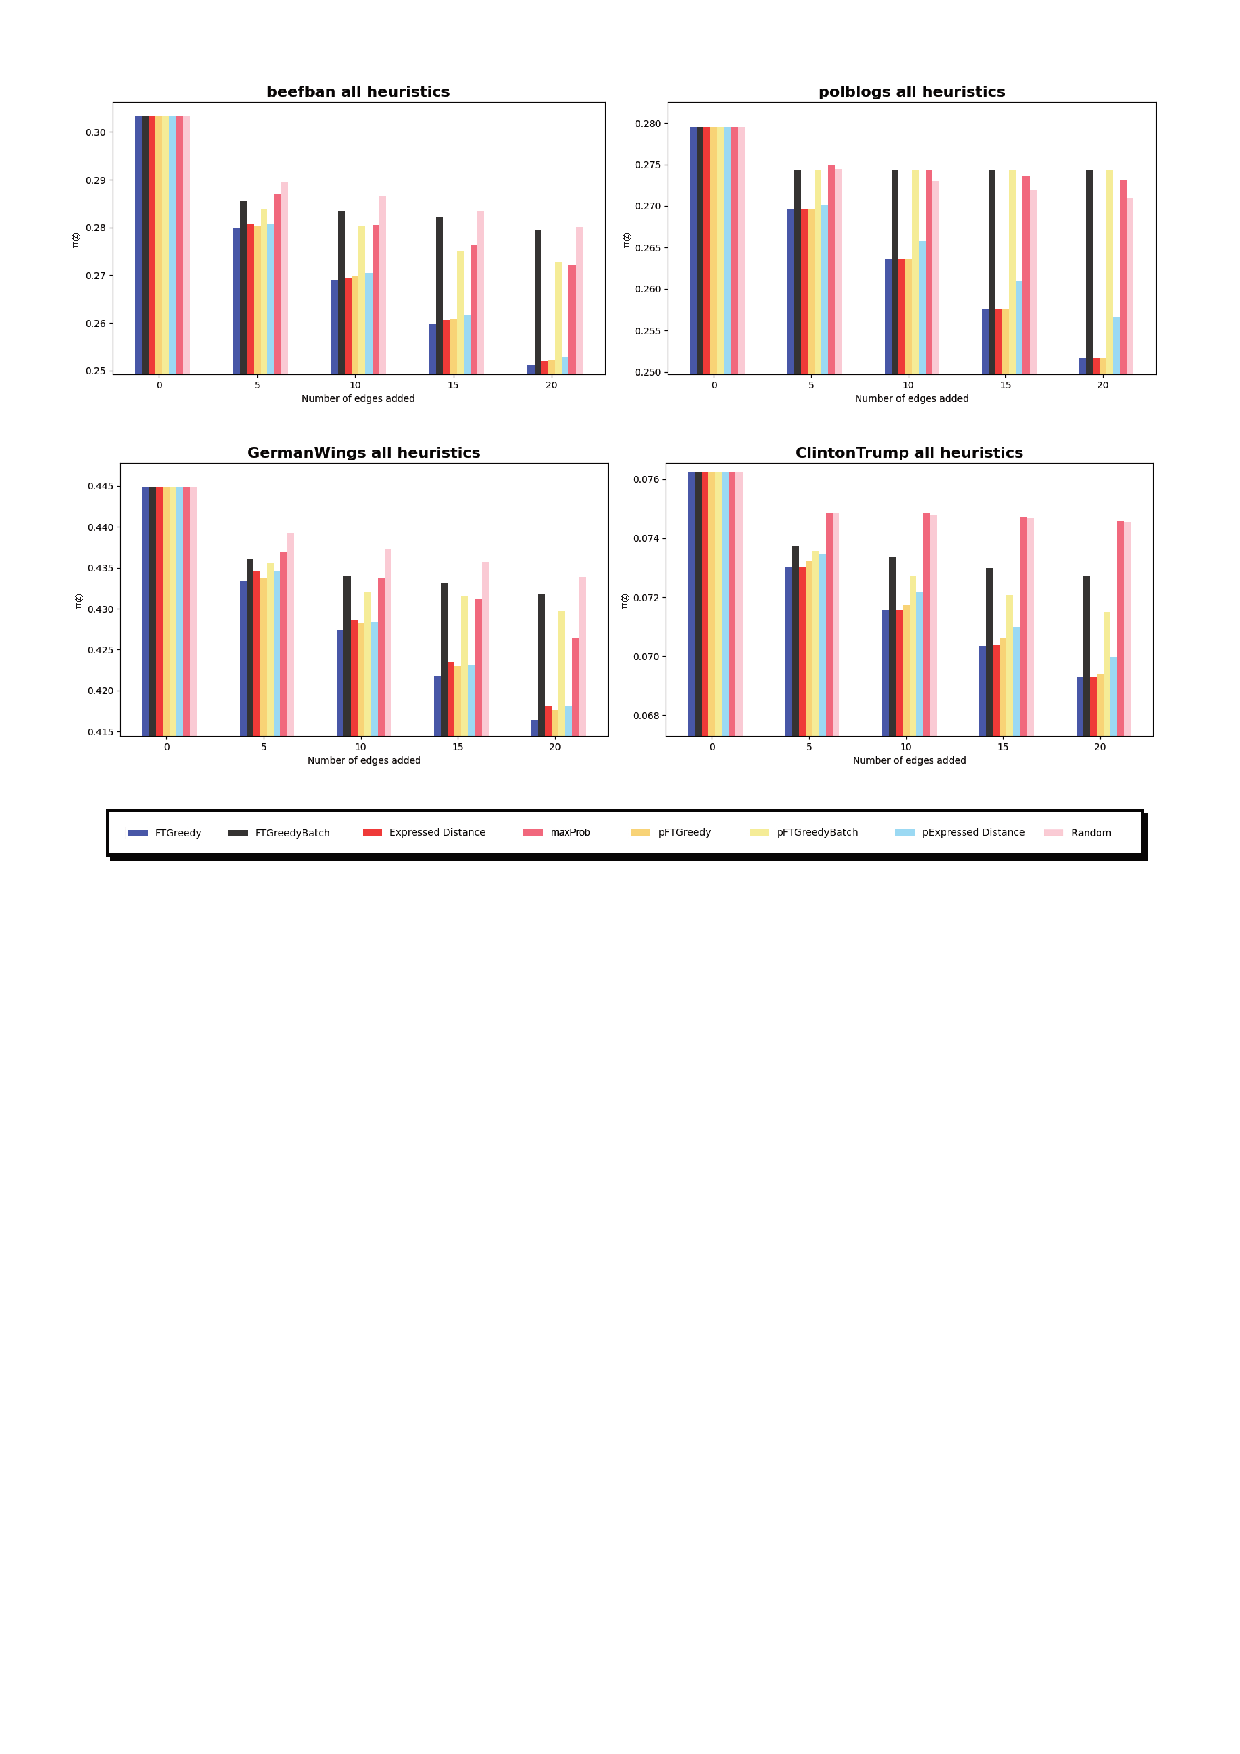
\includegraphics[width=1.2\textwidth]{Figures/all2}
	\caption{Comparison all the heuristics}
	\end{center}
	\label{all2}
\end{figure}







